%--------------------------------------------------------------
% tesi.tex 
%--------------------------------------------------------------
% Corso di Laurea in Informatica 
% http://if.dsi.unifi.it/
% @Facolt\`a di Scienze Matematiche, Fisiche e Naturali
% @Universit\`a degli Studi di Firenze
%--------------------------------------------------------------
% - template for the main file of Informatica@Unifi Thesis 
% - based on Classic Thesis Style Copyright (C) 2008 
%   Andr\'e Miede http://www.miede.de   
%--------------------------------------------------------------

\documentclass[twoside,openright,titlepage,fleqn,
,	headinclude,12pt,a4paper,BCOR5mm,footinclude,table]{scrbook}
%--------------------------------------------------------------
\newcommand{\myItalianTitle}{Utilizzo di un algoritmo Sensor Fusion nell'ambito della localizzazione ferrotramviaria\xspace}
\newcommand{\myEnglishTitle}{Use of a Sensor Fusion Algorithm in the area of tramway localization\xspace}
% use the right myDegree option
\newcommand{\myDegree}{Corso di Laurea in Informatica\xspace}
%\newcommand{\myDegree}{
	%Corso di Laurea Specialistica in Scienze e Tecnologie 
	%dell'Informazione\xspace}
\newcommand{\myName}{Alex Foglia\xspace}
\newcommand{\myProf}{Andrea Bondavalli\xspace}
\newcommand{\myOtherProf}{Nome Cognome\xspace}
\newcommand{\mySupervisor}{Nome Cognome\xspace}
\newcommand{\myFaculty}{
	Scuola di Scienze Matematiche, Fisiche e Naturali\xspace}
\newcommand{\myUni}{\protect{
	Universit\`a degli Studi di Firenze}\xspace}
\newcommand{\myLocation}{Firenze\xspace}
\newcommand{\myTime}{Anno Accademico 2018-2019\xspace}
\newcommand{\myVersion}{Version 0.1\xspace}
%--------------------------------------------------------------

\usepackage[italian]{babel}
\usepackage[latin1]{inputenc}
\usepackage[T1]{fontenc} 
\usepackage[square,numbers]{natbib} 
\usepackage[fleqn]{amsmath}  
\usepackage{ellipsis}
\usepackage{listings}
\usepackage{subfig}
\usepackage{caption}
\usepackage{appendix}
\usepackage{siunitx}
\usepackage{url}

%--------------------------------------------------------------
\usepackage{dia-classicthesis-ldpkg}
%--------------------------------------------------------------


%
% Options for classicthesis.sty:
% tocaligned eulerchapternumbers drafting linedheaders 
% listsseparated subfig nochapters beramono eulermath parts 
% minionpro pdfspacing
\usepackage[eulerchapternumbers,linedheaders,subfig,beramono,eulermath,
parts]{classicthesis}
%--------------------------------------------------------------
\newlength{\abcd} % for ab..z string length calculation
% how all the floats will be aligned
\newcommand{\myfloatalign}{\centering} 
\setlength{\extrarowheight}{3pt} % increase table row height
\captionsetup{format=hang,font=small}
%--------------------------------------------------------------
% Layout setting
%--------------------------------------------------------------
\usepackage{geometry}
\geometry{
	a4paper,
	ignoremp,
	bindingoffset = 1cm, 
	textwidth     = 13.5cm,
	textheight    = 21.5cm,
	lmargin       = 3.5cm, % left margin
	tmargin       = 4cm    % top margin 
}




%%
%% Julia definition (c) 2014 Jubobs
%%
\lstdefinelanguage{Julia}%
  {morekeywords={abstract,break,case,catch,const,continue,do,else,elseif,%
      end,export,false,for,function,immutable,import,importall,if,in,%
      macro,module,otherwise,quote,return,switch,true,try,type,typealias,%
      using,while},%
   sensitive=true,%
   alsoother={},%
   morecomment=[l]\#,%
   morecomment=[n]{\#=}{=\#},%
   morestring=[s]{"}{"},%
   morestring=[m]{'}{'},%
}[keywords,comments,strings]%

\lstset{%
    language         = Julia,
    basicstyle       = \ttfamily,
    keywordstyle     = \bfseries\color{blue},
    stringstyle      = \color{magenta},
    commentstyle     = \color{ForestGreen},
    showstringspaces = false,
}
%%%

\usepackage{tikz}
\usetikzlibrary{arrows}
\usetikzlibrary{positioning}
\tikzset{main node/.style={circle,fill=blue!20,draw,minimum size=1cm,inner sep=0pt},
            }



%--------------------------------------------------------------
\begin{document}
\frenchspacing
\raggedbottom
\pagenumbering{roman}
\pagestyle{plain}
%--------------------------------------------------------------
% Frontmatter
%--------------------------------------------------------------


%--------------------------------------------------------------
% titlepage.tex (use thesis.tex as main file)
%--------------------------------------------------------------
\begin{titlepage}
	\begin{center}
   	\large
      \hfill
      \vfill
      \begingroup
         \includegraphics[scale=0.15]{logo/LOGO}\\
%			\spacedallcaps{\myUni} \\ 
			\myFaculty \\
			\myDegree \\ 
			\myCurriculum \\
			\vspace{0.5cm}
         \vspace{0.5cm}    
           
      \endgroup 
      \vfill 
      \begingroup
      	\color{Maroon}\spacedallcaps{\myItalianTitle} \\ $\ $\\
      	\spacedallcaps{\myEnglishTitle} \\ 	
	\bigskip
      \endgroup
      \spacedlowsmallcaps{\myName} \\ $\ $\\
      \myRel \spacedlowsmallcaps{\myProf}
      \vfill 
      \vfill
    
      \vfill
      \vfill
      \myTime
      \vfill                      
	\end{center}        
\end{titlepage}   
%--------------------------------------------------------------
% back titlepage
%--------------------------------------------------------------
   \newpage
	\thispagestyle{empty}
	\hfill
	\vfill
	\noindent\myName: 
	\textit{\myItalianTitle,} 
	\myDegree, \textcopyright\ \myTime
%--------------------------------------------------------------
% back titlepage end
%--------------------------------------------------------------

\pagestyle{scrheadings}
%--------------------------------------------------------------
% Mainmatter
%--------------------------------------------------------------
\pagenumbering{arabic}
% use \cleardoublepage here to avoid problems with pdfbookmark
%\include{intro} % use \myChapter command instead of \chapter
%\cleardoublepage\myPart{Part I}
%\include{chapter01}
%\cleardoublepage\myPart{Part II}
%\include{chapter02}
%\include{chapter03}
\tableofcontents
\listoftables
\listoffigures
\chapter{Stato dell'Arte}
\section{Introduzione}
Negli ultimi anni, i sistemi informatici hanno assunto un ruolo sempre pi\`u centrale nelle attivit\`a umane.\\*
Inizialmente, il computer era considerato un semplice strumento di supporto alla matematica applicata, capace di svolgere calcoli particolarmente onerosi in un tempo relativamente breve. Con lo sviluppo delle tecnologie, i sistemi informatici sono ad oggi impiegati in un vasto insieme di domini applicativi, dall'elettromedicale al trasporto aereo, fino all'\emph{Internet of Things}.\\*
Quanto pi\`u si diffonde l'utilizzo dei sistemi informatici, tanto pi\`u peso assume un eventuale fallimento dei medesimi.\\*
La letteratura scientifica dimostra che la valutazione della \emph{dependability} di un sistema informatico \`e un problema chiave.\\*
Per \emph{dependability} si intende la capacit\`a che ha un sistema di fornire un servizio in modo corretto. \cite{depdef}\\*
Un \emph{fallimento} \`e una transizione compiuta da un sistema dall'erogazione di un servizio corretto verso l'erogazione di un servizio scorretto. La transizione contraria \`e detta \emph{restauro}.\\*
\begin{figure}[h]
	\centering
	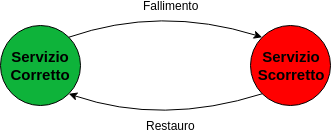
\includegraphics[width=0.7\linewidth]{img/FallimentoRestauro}
	\caption{Fallimento e restauro}
	\label{fig:fallimentorestauro}
\end{figure}\newpage
Effettuare misure sperimentali su un sistema informatico, o su un suo prototipo, \`e una valida opzione per valutarne la \emph{dependability}.\\*
\subsection{Dependability}
La \emph{dependability} di un sistema \`e:
\begin{itemize}
	\item Misurata rispetto a un certo insieme di propriet\`a note come \emph{measures};
	\item Raggiunta attraverso l'utilizzo di specifiche tecniche, i \emph{means};
	\item Minacciata dai \emph{threats}, ossia da tutto ci\`o che porta il sistema ad erogare un servizio improprio.\\*
	Un sistema pu\`o fallire nel caso in cui questo non sia conforme alle specifiche, oppure perch\`e le specifiche non descrivono adeguatamente le sue funzioni.\\*
\end{itemize}
La \emph{dependability} di un sistema viene misurata rispetto alle seguenti propriet\`a:
\begin{itemize}
	\item \emph{Availability}: L'alternanza tra la fornitura di un servizio corretto e uno scorretto.
	$$
	A(t) = \begin{cases} 1 & \mbox{se il servizio fornito \`e corretto al tempo t} \\ 0 & \mbox{altrimenti} \end{cases}
	$$
	$\mathbb E[A(t)]:$ probabilit\`a che il servizio fornito sia corretto al tempo $t$
	\item \emph{Reliability}: Capacit\`a di fornire un servizio continuamente corretto in un certo intervallo di tempo.
	$$
	R(t):\mbox{probabilit\`a di fornire un servizio corretto nell'intervallo }[0,t]
	$$
	\item \emph{Safety}: Il tempo medio a un fallimento catastrofico.\\*\\*
	$S(t):$ probabilit\`a che non si verifichi alcun fallimento catastrofico nell'intervallo $[0,t]$\\*\\*
	\item \emph{Time to Failure}: Il tempo che intercorre fra l'ultimo restauro e il successivo fallimento.\\*
	Spesso \`e opportuno considerare il valore atteso di questa grandezza, il \emph{Mean Time to Failure} (MTTF)
	\item \emph{Maintainability}: Il tempo necessario a restaurare il sistema, dopo l'ultimo fallimento. Il valore atteso di questa misura prende il nome di \emph{Mean Time to Repair} (MTTR)
	\item \emph{Coverage}: Probabilit\`a che il sistema sia in grado di tollerare un guasto.
\end{itemize}
La \emph{safety} \`e un' estensione del concetto di \emph{reliability}.\\*
Si definisce uno stato sicuro in cui il sistema:
\begin{itemize}
	\item Fornisce il servizio corretto, oppure
	\item Non fornisce il servizio corretto, ma il fallimento non ha conseguenze catastrofiche sull'ambiente o sulle persone
\end{itemize}
Qualunque fallimento che induca il sistema a fornire un servizio scorretto con conseguenze catastrofiche, viene modellato come una transizione verso uno stato non sicuro. Quando esiste questa possibilit\`a, il sistema viene definito \emph{safety-critical}.\cite{safetycritical}\\*
\begin{figure}[h]
	\centering
	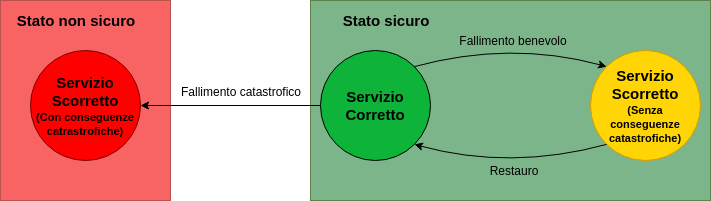
\includegraphics[width=0.7\linewidth]{img/safety}
	\caption{La \emph{safety} estende il concetto di \emph{reliability}}
	\label{fig:safety}
\end{figure}\\*
Esistono numerosi contesti in cui i sistemi impiegati vengono definiti \emph{safety-critical}, uno di questi \`e il trasporto ferroviario.\\*
I \emph{threats} che minano la \emph{dependability} di un sistema sono i guasti, gli errori e i fallimenti.\\*
Un guasto \`e un qualunque evento interno al sistema in grado di causare un errore. Quando l'errore raggiunge l'interfaccia di servizio, ovvero altera il servizio fornito dal sistema, si parla di fallimento. In letteratura, si fa riferimento a questo rapporto di causalit\`a come \emph{fault error failure chain}, catena guasto errore fallimento.\\*
\begin{figure}[h]
	\centering
	
\includegraphics[width=0.7\linewidth]{img/gefpng}
	\caption{Catena guasto errore fallimento}
	\label{fig:gefpng}
\end{figure}\newpage
La \emph{dependability} di un sistema informatico \`e raggiunta attraverso l'uso di quattro tecniche:
\begin{itemize}
	\item \emph{Fault Prevention}: Previene l'insorgenza di guasti durante il ciclo di vita del sistema;
	\item \emph{Fault Tolerance}: Rende il sistema in grado di fornire un servizio corretto anche in presenza di guasti;
	\item \emph{Fault Removal}: Riduce il numero di guasti nel sistema;
	\item \emph{Fault Forecasting}: Stima il numero di guasti presenti nel sistema, attualmente o in futuro;
\end{itemize}
La \emph{dependability} \`e la propriet\`a che viene misurata durante il processo di \emph{validazione}.\\*
La validazione \`e un processo atto a determinare se il sistema \`e conforme alle sue specifiche funzionali.\\*
Il processo di validazione avviene durante tutte le fasi del ciclo di vita del sistema, anche prima che venga realizzato. Per questo motivo, il sistema viene opportunamente modellato al fine di condurre propriamente l'analisi.\\*
\begin{figure}[h]
	\centering
	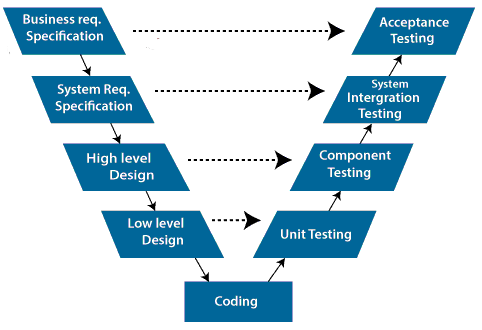
\includegraphics[width=0.7\linewidth]{img/vmodel}
	\caption{Il ciclo di vita dei sistemi: modello a V}
	\label{fig:vmodel}
\end{figure}
\noindent{}A discrezione della fase del ciclo di vita del sistema, si utilizzano differenti tecniche e modelli di validazione: \cite{librobonda}
\begin{itemize}
	\item Specifica: la validazione \`e basata sull'utilizzo di tecniche combinatorie che mirano a determinare le condizioni di fallimento di un sistema in funzione del fallimento dei suoi sottocomponenti, considerati indipendenti;
	\item \emph{Design}: in questa fase si usano modelli analitici \emph{state-based} basati su processi casuali, come ad esempio le Catene di Markov. Si rilassano le assunzioni di indipendenza tipiche dei modelli combinatori;
	\item Implementazione: con il procedere della fase di implementazione, il sistema prende forma e pu\`o essere interessante osservarne direttamente il comportamento per effettuare misure sperimentali. L'attivit\`a di osservazione e misurazione prende il nome di \emph{monitoring};
	\item Fase operativa: il sistema \`e impiegato sul campo e possono essere utilizzate tutte le tecniche disponibili per l'analisi.
\end{itemize}
\subsection{Osservazione dei sistemi}
L'osservazione, o \emph{monitoring}, \`e una tecnica per valutare la \emph{dependability} di un sistema o un suo prototipo osservandone l'esecuzione nell'ambiente finale.\\*
In questa sezione viene esposto il \emph{monitoring} dei sistemi informatici come descritto nei lavori \cite{monitor1}, \cite{monitor2} e \cite{monitor3}.\\*
L'obiettivo \`e quello di monitorare costantemente l'esecuzione del sistema, verificando che il comportamento osservato sia confrome alle aspettative.\\*
Un'attivit\`a di \emph{monitoring} \`e seguita da un'attivit\`a di verifica. Questa pu\`o essere fatta durante l'esecuzione del sistema oppure \emph{offline}, esaminando successivamente i risultati.\\*
Il \emph{monitoring} \`e stato riconosciuto come una valida opzione per valutare gli attributi di \emph{dependability} dei sistemi informatici.\\*
I problemi tecnici da affrontare e risolvere quando si crea un sistema di \emph{monitoring} riguardano:
\begin{itemize}
	\item Individuazione e classificazione degli eventi di interesse, al fine di raccogliere misurazioni utili per valutare correttamente la \emph{dependability} del sistema monitorato;
	\item Trasmissione delle informazioni al luogo dove queste saranno elaborate;
	\item Filtraggio e classificazione degli eventi rispetto alle misure di interesse.
\end{itemize}
Si definisce \emph{target system} il sistema al quale vengono applicate le attivit\`a di \emph{monitoring}. Il componente hardware o software interno al sistema verso il quale si riferisce il \emph{monitoring}, viene detto \emph{target component} o \emph{target application}.\\*
Esistono due differenti configurazioni di un processo di monitoring: \emph{black-box} o \emph{white-box}. Nella configurazione a \emph{black-box} il sistema viene sottoposto a un certo carico di input al fine di osservare l'output prodotto. L'input fornito al sistema prende il nome di \emph{workload}, ed \`e il carico di informazioni che il sistema dovr\`a processare durante il \emph{monitoring}.\\*
\begin{figure}[h]
	\centering
	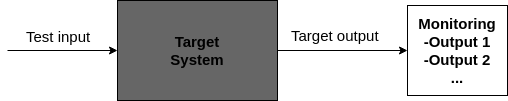
\includegraphics[width=0.7\linewidth]{img/blackbox}
	\caption{Monitoring black-box}
	\label{fig:blackbox}
\end{figure}
\FloatBarrier
Il monitoring \emph{white-box} prevede l'utilizzo agiuntivo di strumenti necessari a osservare anche gli output intermedi che il sistema produce. Questi strumenti sono chiamati sonde, o \emph{probes}.\\*
\begin{figure}[h]
	\centering
	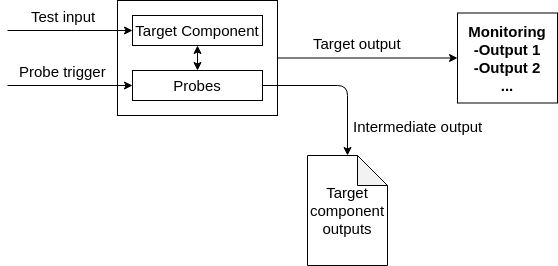
\includegraphics[width=0.7\linewidth]{img/whitebox}
	\caption{Monitoring white-box}
	\label{fig:whitebox}
\end{figure}
\FloatBarrier
I \emph{probes} sono collocati solitamente all'interno del sistema e il loro scopo \`e quello di fornire informazioni pi\`u dettagliate sul comportamento del \emph{target component}.\\*
Se si vogliono monitorare segnali hardware interni al sistema, i \emph{probes} utilizzati saranno effettivamente hardware, mentre si utilizzano \emph{probe} software se si vuole ottenere informazioni sull'esecuzione interna di un programma. Questa tecnica \`e chiamata instrumentazione del codice, e il codice aggiunto prende il nome di \emph{software probe}.\\*
Quando si progetta il \emph{monitoring} di un sistema, si devono rispettare due regole principali:
\begin{itemize}
	\item I \emph{probes} devono essere in grado di raccogliere il giusto numero di informazioni circa il comportamento del sistema;
	\item Il comportamento del \emph{target system} non deve essere alterato in maniera significativa a causa dell'inserimento dei \emph{probes}. Quando questo avviene, si dice che il sistema di monitoraggio \`e \emph{poco intrusivo}.
\end{itemize}
\subsection{Fault Injection}
La \emph{fault injection} \`e un approccio all'analisi della \emph{dependability} che estende le tecniche di \emph{monitoring} esposte in 1.1.2.\\*
\`E definita come la volontaria introduzione di guasti all'interno di un sistema, al fine di osservarne il comportamento in presenza di guasti. \cite{faultinj1} \cite{faultinj2} \cite{faultinj3}\\*

\section{Scopo della Tesi}
Questa Tesi descrive l'attivit\`a di \emph{monitoring} del prototipo di un sistema informatico impiegato nell'ambito del posizionamento ferrotramviario. Per quanto esposto in 1.1.1, il dominio ferrotramviario \`e un contesto \emph{safety-critical}, come tale, lo sviluppo di sistemi informatici da impiegare nell'ambito ferrotramviario \`e regolamentato da specifici standard e requisiti di \emph{dependability}.\\*
Si introducono i sistemi ferrotramviari come derivazione dai classici sistemi ferroviari, si descrive il problema del posizionamento e le tecniche attualmente utilizzate per risolverlo, inquadrando il contesto operativo in cui si colloca il sistema analizzato.
\section{Sistemi Ferroviari e Ferrotramviari}
\`E possibile schematizzare un sistema ferroviario, o ferrotramviario, come un insieme di vetture vincolate a muoversi lungo una traccia fissata.\\*
Questa schematizzazione \`e approssimativamente valida per qualsiasi sistema ferroviario o ferrotramviario, a prescindere dal numero di veicoli transitanti o dall'estensione geografica. Ci\'o che invece differenzia un sistema ferroviario da un sistema ferrotramviario sono:
\begin{itemize}
		\item Le caratteristiche fisiche del veicolo transitante, come lunghezza e massa;
		\item Le caratteristiche geografiche dell'ambiente operativo;
		\item Gli scopi del trasporto.
\end{itemize}
In generale, nel trasporto ferroviario si utilizzano veicoli pesanti atti a trasportare persone o merci su lunghe percorrenze, pertanto \`e comune che l'ambiente operativo di un sistema ferroviario sia prevalentemente extra urbano.\\*
Nel trasporto ferrotramviario, di contro, si utilizzano veicoli leggeri per offrire un'alternativa al cittadino all'utilizzo di mezzi privati durante i suoi spostamenti all'interno di un'area metropolitana. Quest'ultima caratteristica implica che l'ambiente operativo di un sistema ferrotramviario sia radicalmente diverso dall'ambiente operativo di un sistema ferroviario. Le vetture, anche dette \emph{rotabili}, si muovono lungo traccie installate su strade urbane, e di conseguenza il traffico ferrotramviario condivide l'ambiente con il traffico cittadino, come mostrato in figura \ref{fig:tramschema}.\\*
\begin{figure}[h]
		\centering
		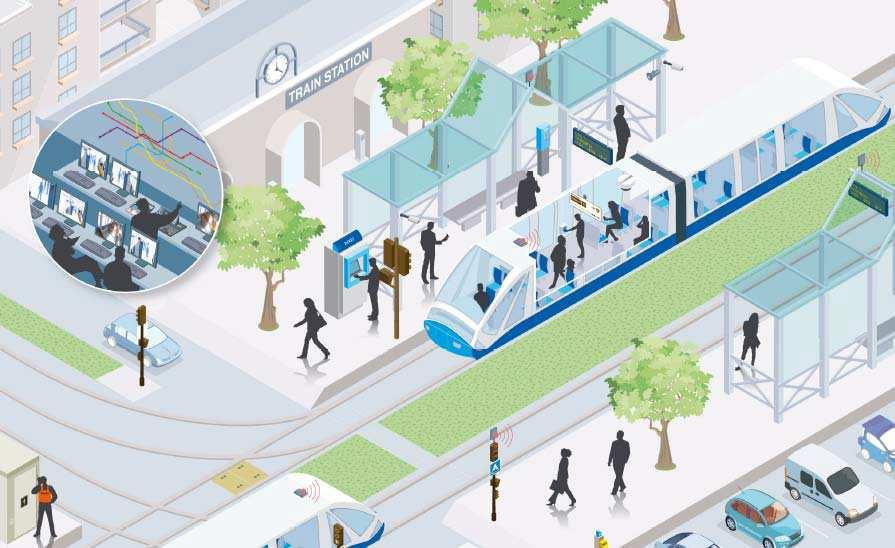
\includegraphics[width=0.7\linewidth]{img/twschema}
		\caption{Schema di un tipico scenario ferrotramviario}
		\label{fig:tramschema}
\end{figure}
\subsection{La safety nei sistemi ferroviari}
La gestione della \emph{safety} nei sistemi ferroviari \`e regolamentata dallo standard \texttt{EN 50126}. \cite{50126}\\*
Questo standard definisce un insieme di documenti che regolamentano la gestione della \emph{safety} nel dominio ferroviario, con particolare enfasi verso le attivit\`a di valutazione RAMS (\emph{Reliability, Availability, Maintainability, Safety}).\\*
Esso prevede che vengano redatti i seguenti documenti.
\paragraph{Safety Plan}\mbox{}\\*Un insieme documentato di attivit\`a programmate, risorse ed eventi necessari a implementare la struttura organizzativa, le responsabilit\`a, le procedure, le attivit\`a, le funzioni e le risorse che insieme assicurano la \emph{safety} del sistema.\\*
In sintesi, il \emph{safety plan} individua \emph{chi} fa \emph{cosa}, e \emph{quando}, al fine di realizzare un sistema \emph{safe}.
\paragraph{Safety Requirements}\mbox{}\\*Definisce i requisiti di \emph{safety} che il sistema deve soddisfare prima di poter essere impiegato sul campo.
\paragraph{Safety Case}\mbox{}\\*La dimostrazione documentata che un prodotto sia conforme ai suoi requisiti di \emph{safety}.
Il \emph{Safety Case} deve essere redatto come una dimostrazione logica della \emph{safety} del sistema.\\*\\*Per quanto riguarda le procedure e i requisiti tecnici per lo sviluppo di applicazioni software utilizzate nel controllo ferroviario, lo standard di riferimento \`e \texttt{EN 50128}. \cite{50128}\\*
Lo standard \texttt{EN 50128} impone che a ciascun software integrato all'interno di un sistema ferroviario debba essere assegnato un livello di \emph{Safety Integrity Level} (SIL). \cite{sil}\\*
Il livello SIL viene assegnato sulla base del tempo medio al fallimento catastrofico, ossia il MTTF relativo a fallimenti catastrofici.\\*
\begin{table}[h]
	\centering
	\begin{tabular}{|l|l|}
		\hline 
		\textbf{Livello SIL} & \textbf{Tempo medio al fallimento catastrofico} \\ 
		\hline 
		\texttt{SIL-1} & $[10^5 - 10^6)$ ore \\ 
		\hline 
		\texttt{SIL-2} & $[10^6 - 10^7)$ ore \\ 
		\hline 
		\texttt{SIL-3} & $[10^7 - 10^8)$ ore \\ 
		\hline 
		\texttt{SIL-4} & $\ge 10^8$ ore \\ 
		\hline 
	\end{tabular} 
\caption{Livelli SIL}
\end{table}
\FloatBarrier
\noindent{}Mentre lo standard \texttt{EN 50126} \`e generico e applicabile a qualunque sistema ferroviario o parti di esso, poich\`e relativo alla \emph{gestione} della \emph{safety} piuttosto che al suo effettivo raggiungimento, lo standard \texttt{EN 50128} \`e inerentemente tecnico e specifico per i software critici.\\*Esso identifica le fasi principali nel ciclo di vita del software e per ciascuna di queste prevede un insieme di tecniche da utilizzare per soddisfare il SIL assegnato al software.
\section{Il problema del posizionamento}
Per posizionamento ferroviario si intende la valutazione della posizione di un treno all'interno di una traccia ferroviaria. Tale posizione viene espressa come progressiva chilometrica rispetto a una posizione nota, come ad esempio l'origine della linea. \cite{trainpositioning}\\*
\subsubsection{Odierne Tecniche di Posizionamento}
Gli odierni sistemi di posizionamento si basano principalmente sull'utilizzo di strumenti installati a terra, chiamati \emph{beacon}, o \emph{balise} in gergo ferroviario, i quali hanno lo scopo di rilevare il passaggio di un treno.\cite{tecnicheodierne}
Esiste uno standard a livello europeo al quale gli odierni sistemi di posizionamento si devono uniformare, l' \emph{European Train Control System} (ETCS).\\*
Nel corso della storia, ogni paese europeo ha sviluppato autonomamente le proprie infrastrutture ferroviarie e relative regole operative. Tuttavia, ad oggi i treni possono attraversare le frontiere, pertanto \`e necessario sviluppare un sistema ferroviario standard che rispetti una comune normativa operazionale europea. Tale sistema prende il nome di \emph{European Rail Traffic Management System} (ERTMS) \cite{ertms}, ed ETCS \`e il sottosistema di ERTMS dedicato al posizionamento delle vetture.\\*
Come standard, ETCS definisce specifici livelli di \emph{compliance} che possiede un sistema di posizionamento rispetto ad ETCS, ed essi vanno dal livello \texttt{ETCS-0} al livello \texttt{ETCS-3}.\\*
L'obiettivo \`e quello di sviluppare progressivamente un sistema di posizionamento completamente autonomo (\texttt{ETCS-3}), partendo da un sistema interamente \emph{non-compliant} con ETCS (\texttt{ETCS-0}).
\\*
Allo stato attuale, quasi tutti i sistemi di posizionamento sono \texttt{ETCS-2}. Nei livelli \texttt{ETCS-1} e \texttt{ETCS-2}, le traccie vengono suddivise in blocchi, e all'entrata di ciascun blocco viene posizionato un \emph{beacon} in grado di rilevare la presenza di un treno.\\*
L'autorizzazione all'ingresso in un blocco viene rilasciata se nessun altro treno sta occupando il blocco al quale si vuole accedere, mentre un sistema di \emph{odometria} installato a bordo, posiziona il treno rispetto all'ultimo \emph{beacon} incontrato.\\*
Nel livello \texttt{ETCS-3}, non sono richiesti segnali provenienti dalla linea: un treno deve essere in grado di posizonarsi autonomamente. \cite{etcs3}\\*
In sintesi, i livelli ETCS possono essere descritti come segue:
\begin{itemize}
	\item \texttt{ETCS-0}: Sistema non conforme a ETCS;
	\item \texttt{ETCS-1}: Utilizzo di apparati di posizionamento installati a terra, autorizzazione a procedere segnalata al macchinista attraverso indicazioni semaforiche;
	\item \texttt{ETCS-2}: Come \texttt{ETCS-1}, ma l'autorizzazione a procedere \`e gestita da un sistema automatico di scambio, denominato sistema di \emph{interlocking};\cite{interlocking}
	\item \texttt{ETCS-3}: Posizionamento autonomo, nessun utilizzo di apparati a terra.
\end{itemize}
\begin{figure}[h]
	\centering
	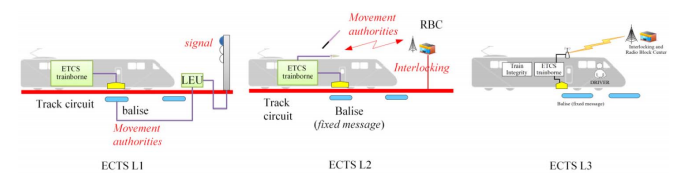
\includegraphics[width=\linewidth]{img/etcs123.png}
	\caption{Livelli \texttt{ETCS}}
	\label{fig:etcs123}
\end{figure}
Il livello \texttt{ETCS-2} prevede che l'autorizzazione a procedere venga gestita dal sistema di \emph{interlocking} e non dal solo operatore umano notificato mediante indicazioni semaforiche.\\*
La funzionalit\`a offerta del sistema di \emph{interlocking} viene pertanto considerata \emph{safety-critical}, in quanto un suo fallimento pu\`o portare a conseguenze anche catastrofiche.\cite{marocchini}\\*
ETCS adotta un approccio incrementale alla realizzazione di sistemi di posizionamento autonomi. Un sistema di posizionamento \texttt{ETCS-3} deve continuare a interagire con il sistema di \emph{interlocking}, quindi deve essere considerato a sua volta un sistema \emph{safety-critical}.\\*
ERTMS/ETCS \`e pensato per sistemi ferroviari, mentre nel dominio ferrotramviario vige la regola della \emph{marcia a vista}. Il rispetto di ETCS non \`e obbligatorio in detto contesto, tuttavia le tecniche di posizionamento ivi utilizzate rispettano spesso le linee guida imposte da ETCS. 
\subsection{Verso ETCS-3}
Gli attuali sistemi di posizionamento richiedono un minimo intervento di computer installati a bordo e una grande quantit\`a di apparati installati a terra. Gli apparati di terra sono costosi e hanno un impatto ambientale non trascurabile, pertanto \`e necessario iniziare a pianificare una migrazione verso sistemi \texttt{ETCS-3}.\cite{market}\\*
Il sistema analizzato in questa Tesi \`e un sottosistema di posizionamento conforme alla filosofia \texttt{ETCS-3}.
\section{Definizione del problema affrontato}
Nell'ottica di migrazione verso sistemi \texttt{ETCS-3}, \`e stato progettato un sistema di posizionamento ferrotramviario autonomo, basato principalmente sull'utilizzo di un \emph{sensore inerziale} installato a bordo treno, le cui misurazioni vengono processate da un sistema software. \cite{svolta}\\*
Attualmente il sistema ha superato le fasi di analisi e definizione dei requisiti, \emph{system design}, e si trova nella fase di implementazione. Si \`e quindi reso disponibile per l'analisi di \emph{dependability} un prototipo del sistema.\\*
Per quanto esposto in 1.1.1, questo pu\`o essere osservato durante l'esecuzione nel suo ambiente operativo.







%--------------------------------------------------------------
\end{document}
%--------------------------------------------------------------